% Provenance (never printed): old premiere S / seconde material on minerals and
% rocks (identifying minerals in hand specimen, the silicates, the minerals of
% granite, basalt and peridotite, thin sections in polarised light).
% Element fractions and rock densities from figdata/grade-11/mineral_density.py
% (Rudnick and Gao 2014 bulk crust; webmineral mean densities). Mineral, crystal,
% rock families and the Mohs scale are Book 1's (grade 6): recalled, not defined.
% Felsic and mafic belong to g11.08: not used here.
\chapter{Los minerales}\label{ch:g11:minerals}

Toma un canto de granito y míralo con una lupa. No es una sola sustancia,
sino un mosaico de granos trabados entre sí: granos grises, vítreos y casi
transparentes; granos rosados, macizos, cuyas caras rotas destellan a la luz
cuando se gira el canto; pequeñas escamas negras que la punta de un cuchillo
levanta en láminas finas. Cada tipo de grano es un mineral. Este capítulo
muestra cómo los distingue un geólogo, por qué casi todos están construidos
con silicio y oxígeno, cómo forman las rocas que ya han aparecido ---granito,
basalto, peridotita--- y cómo una lámina de roca más fina que un cabello,
vista con luz polarizada, los muestra todos a la vez.

\begin{omfigure}
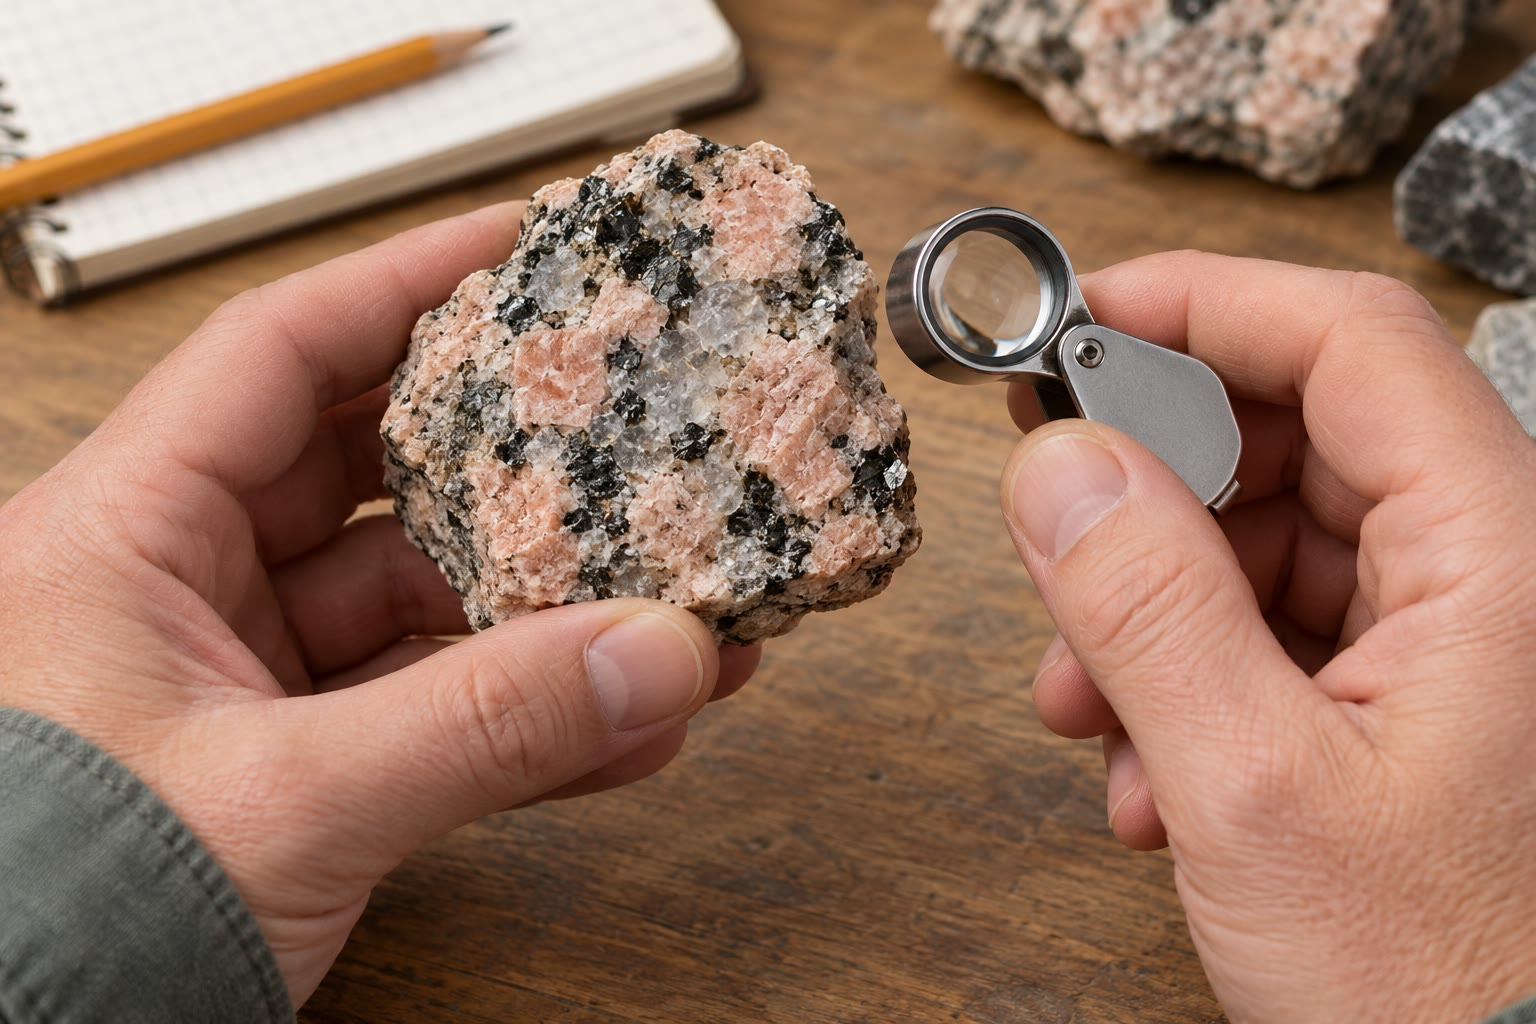
\includegraphics[width=0.62\linewidth]{images/book2/ai/g11-geologist-hand-lens.jpg}

{\small Un granito examinado con una lupa: la primera herramienta para
distinguir los minerales. (Ilustración generada por IA.)}
\end{omfigure}

\begin{recall}
Un mineral es una sustancia sólida natural, no fabricada por seres vivos, de
composición fija y con sus átomos ordenados de forma regular; una roca está
formada por uno o varios minerales. El granito está formado sobre todo por
feldespato, cuarzo y mica. Las rocas se reparten en tres familias: ígneas,
sedimentarias y metamórficas. La dureza de un mineral es su resistencia a ser
rayado, clasificada de 1 (talco) a 10 (diamante) en la escala de Mohs; el
feldespato ortosa tiene 6 y el cuarzo 7, mientras que una placa de vidrio
tiene alrededor de 5.5 y un clavo de acero alrededor de 6.5 (Libro 1, año 6).
La densidad de un cuerpo es su masa dividida entre su volumen (los libros de
física). Un compuesto se describe con una fórmula que cuenta sus átomos; en un
sólido formado por iones, las cargas positivas y negativas se compensan (los
libros de química). La \omterm{def:g11:ocean-ridges:peridotite}{peridotita} forma el manto; el \omterm{def:g11:ocean-ridges:gabbro}{gabro} y el basalto forman
la \omterm{def:g11:ocean-ridges:oceanic-lithosphere}{corteza oceánica} (el \cref{ch:g11:ocean-ridges}).
\end{recall}
% ledger: usgs:mineral-rock, nps:granite-minerals, nps:mohs-ladder, nps:mohs-testers

\section{Distinguir los minerales}

Un mineral tiene una composición fija y una ordenación regular de sus átomos.
Las dos se notan por fuera: en la forma de sus cristales, en cómo se rompe, en
cómo refleja la luz, en su dureza y en su densidad. Ninguna de estas
propiedades basta por sí sola; juntas identifican los minerales comunes en
muestra de mano, sin más instrumentos que una lupa, un clavo de acero y una
placa de vidrio.

\paragraph{La forma.} Un cristal que creció libremente, en una cavidad o en un
líquido, adopta una forma que refleja la ordenación de sus átomos.

\begin{definition}[Hábito]\label{def:g11:minerals:habit}
El \emph{hábito}\index{habito (de un cristal)@hábito (de un cristal)} de un mineral es la forma general
que adoptan sus cristales: cúbico, tabular (plano, como una tableta),
prismático (alargado, como un prisma), hojoso, acicular (en forma de aguja),
etcétera.
\end{definition}
% ledger: tulane:physprop

El cuarzo crece en prismas de seis caras terminados en punta; la biotita, en
placas planas de seis lados (fotografías siguientes). En la mayoría de las
rocas, sin embargo, los granos crecieron unos contra otros y no tienen caras
propias: el \omterm{def:g11:minerals:habit}{hábito} dice entonces poco, y toman el relevo las demás
propiedades.
% ledger: photo:g11-quartz, photo:g11-biotite

\paragraph{El color y el brillo.} El color es lo primero que se ve, y lo menos
fiable. Basta una traza de otro elemento para cambiarlo: el cuarzo puede ser
incoloro, blanco, negro, rosa, azul o violeta. En cambio, unos pocos minerales
apenas varían: el olivino es casi siempre verde. La forma en que un mineral
refleja la luz es una guía mejor.
% ledger: tulane:physprop

\begin{definition}[Brillo]\label{def:g11:minerals:lustre}
El \emph{brillo}\index{brillo} de un mineral es su aspecto con luz reflejada.
Es \emph{metálico} cuando el mineral reluce como un metal, y no metálico en
los demás casos: \emph{vítreo} (como el vidrio, igual que el cuarzo),
nacarado, resinoso, etcétera.
\end{definition}
% ledger: tulane:physprop

\paragraph{Cómo se rompe.} Si se golpea un cristal, se rompe. Donde los
enlaces entre sus átomos son más débiles a lo largo de ciertos planos, se
parte a lo largo de ellos, una y otra vez, en superficies planas y brillantes;
donde ningún plano es más débil que otro, se rompe según cualquier superficie.

\begin{definition}[Exfoliación; fractura]\label{def:g11:minerals:cleavage}
La \emph{exfoliación}\index{exfoliacion (de un mineral)@exfoliación (de un mineral)} es la tendencia de un
mineral a romperse según planos lisos, paralelos a direcciones en las que los
enlaces entre sus átomos son más débiles. La \emph{fractura}\index{fractura (de un mineral)}
es la rotura según superficies irregulares, en un mineral sin ningún plano de
debilidad; una fractura de superficies curvas y lisas, como la del vidrio
roto, se llama \emph{concoidea}.
\end{definition}
% ledger: tulane:physprop

Un mineral puede tener una \omterm{def:g11:minerals:cleavage}{exfoliación}, dos, tres o ninguna. Las micas tienen
una, perfecta: se separan en láminas. Los feldespatos tienen dos. El cuarzo no
tiene ninguna: se rompe con una \omterm{def:g11:minerals:cleavage}{fractura} concoidea, lo que lo distingue enseguida
de un feldespato del mismo color gris o blanco. El ángulo entre dos
exfoliaciones lo fija la ordenación de los átomos, y puede medirse en un grano
roto o en un corte: las dos exfoliaciones de un piroxeno se cortan a unos
\ang{87} y \ang{93}, casi en ángulo recto; las de un anfíbol, a unos \ang{56} y
\ang{124}. Los piroxenos y los anfíboles suelen ser oscuros y parecidos; sus
ángulos de \omterm{def:g11:minerals:cleavage}{exfoliación} los distinguen.
% ledger: wm:densities (quartz conchoidal; orthoclase two cleavages; biotite one), tulane:cleavage-angles

\begin{omfigure}
\begin{tikzpicture}[font=\footnotesize]
  % pyroxene: octagonal cross-section, cleavage traces at 46.5 and 133.5 degrees (87/93)
  \begin{scope}
    \coordinate (p1) at (1,0.4); \coordinate (p2) at (0.431,1); \coordinate (p3) at (-0.431,1);
    \coordinate (p4) at (-1,0.4); \coordinate (p5) at (-1,-0.4); \coordinate (p6) at (-0.431,-1);
    \coordinate (p7) at (0.431,-1); \coordinate (p8) at (1,-0.4);
    \begin{scope}[scale=1.5]
      \fill[black!72!green!40] (1,0.4) -- (0.431,1) -- (-0.431,1) -- (-1,0.4) -- (-1,-0.4) -- (-0.431,-1) -- (0.431,-1) -- (1,-0.4) -- cycle;
      \clip (1,0.4) -- (0.431,1) -- (-0.431,1) -- (-1,0.4) -- (-1,-0.4) -- (-0.431,-1) -- (0.431,-1) -- (1,-0.4) -- cycle;
      \foreach \s in {-5,...,5} {
        \draw[white!85!black, line width=0.5pt] ($(136.5:\s*0.24)+(46.5:-3)$) -- ($(136.5:\s*0.24)+(46.5:3)$);
        \draw[white!85!black, line width=0.5pt] ($(223.5:\s*0.24)+(133.5:-3)$) -- ($(223.5:\s*0.24)+(133.5:3)$);}
      \draw[black!80, line width=0.9pt] (46.5:-3) -- (46.5:3); \draw[black!80, line width=0.9pt] (133.5:-3) -- (133.5:3);
    \end{scope}
    \draw[black!70, line width=0.7pt, scale=1.5] (1,0.4) -- (0.431,1) -- (-0.431,1) -- (-1,0.4) -- (-1,-0.4) -- (-0.431,-1) -- (0.431,-1) -- (1,-0.4) -- cycle;
    \draw[omProp, line width=1pt] (46.5:0.75) arc[start angle=46.5, end angle=133.5, radius=0.75];
    \draw[omDef, line width=1pt] (133.5:0.5) arc[start angle=133.5, end angle=226.5, radius=0.5];
    \node[fill=white, inner sep=1pt, text=omProp!80!black] at (90:0.98) {\ang{87}};
    \node[fill=white, inner sep=1pt, text=omDef] at (180:0.82) {\ang{93}};
    \node[anchor=north, align=center] at (0,-1.7) {\strut\textbf{piroxeno}\\exfoliaciones a unos \ang{87} y \ang{93}};
  \end{scope}
  % amphibole: elongated hexagon, cleavage traces at 28 and 152 degrees (56/124 opening sideways)
  \begin{scope}[xshift=6.2cm]
    \begin{scope}[scale=1.5]
      \fill[black!72!green!40] (1.6,0) -- (0.62,0.52) -- (-0.62,0.52) -- (-1.6,0) -- (-0.62,-0.52) -- (0.62,-0.52) -- cycle;
      \clip (1.6,0) -- (0.62,0.52) -- (-0.62,0.52) -- (-1.6,0) -- (-0.62,-0.52) -- (0.62,-0.52) -- cycle;
      \foreach \s in {-6,...,6} {
        \draw[white!85!black, line width=0.5pt] ($(118:\s*0.2)+(28:-4)$) -- ($(118:\s*0.2)+(28:4)$);
        \draw[white!85!black, line width=0.5pt] ($(242:\s*0.2)+(152:-4)$) -- ($(242:\s*0.2)+(152:4)$);}
      \draw[black!80, line width=0.9pt] (28:-4) -- (28:4); \draw[black!80, line width=0.9pt] (152:-4) -- (152:4);
    \end{scope}
    \draw[black!70, line width=0.7pt, scale=1.5] (1.6,0) -- (0.62,0.52) -- (-0.62,0.52) -- (-1.6,0) -- (-0.62,-0.52) -- (0.62,-0.52) -- cycle;
    \draw[omProp, line width=1pt] (-28:0.75) arc[start angle=-28, end angle=28, radius=0.75];
    \draw[omDef, line width=1pt] (28:0.42) arc[start angle=28, end angle=152, radius=0.42];
    \node[fill=white, inner sep=1pt, text=omProp!80!black] at (0:1.02) {\ang{56}};
    \node[fill=white, inner sep=1pt, text=omDef] at (90:0.6) {\ang{124}};
    \node[anchor=north, align=center] at (0,-1.7) {\strut\textbf{anfíbol}\\exfoliaciones a unos \ang{56} y \ang{124}};
  \end{scope}
\end{tikzpicture}

{\small Secciones transversales de un cristal de piroxeno (izquierda) y de un
cristal de anfíbol (derecha), cortados perpendicularmente a su longitud (un
dibujo). Las líneas finas son las trazas de las dos exfoliaciones, dos de
ellas dibujadas más gruesas donde se leen los ángulos; los ángulos entre ellas, casi rectos en el piroxeno, mucho más abiertos y mucho más cerrados en el anfíbol, distinguen
dos minerales oscuros por lo demás parecidos.}
\end{omfigure}
% ledger: tulane:cleavage-angles

\paragraph{La dureza y la densidad.} La dureza, que ya apareció en el Libro 1,
separa minerales de aspecto parecido: el cuarzo (7) raya el vidrio y no lo
raya un clavo de acero; un feldespato (6) también raya el vidrio, pero el
clavo lo raya. La densidad es la última pista. En la mano no puede pesarse un
grano, pero sí una muestra de un solo mineral, y los minerales comunes de las
rocas abarcan un intervalo estrecho, de unos \qty{2.6}{g/cm^3} a unos
\qty{3.4}{g/cm^3} (gráfica siguiente): los más ligeros son ricos en silicio,
aluminio, sodio y potasio, y los más densos, en hierro y magnesio.
% ledger: nps:mohs-ladder, nps:mohs-testers, wm:densities

\begin{method}[Identificar un mineral en muestra de mano]\label{met:g11:minerals:identify}
\begin{enumerate}
  \item Observa la forma del grano o del cristal (\omterm{def:g11:minerals:habit}{hábito}), su color ---solo
        como indicio--- y su \omterm{def:g11:minerals:lustre}{brillo}.
  \item Busca la \omterm{def:g11:minerals:cleavage}{exfoliación}: superficies planas y brillantes que reflejan la
        luz a la vez cuando se gira la muestra. Cuenta las direcciones de
        \omterm{def:g11:minerals:cleavage}{exfoliación} y estima el ángulo entre ellas; si no hay ninguna,
        describe la \omterm{def:g11:minerals:cleavage}{fractura}.
  \item Prueba la dureza con objetos de referencia: una placa de vidrio
        (alrededor de 5.5) y un clavo de acero (alrededor de 6.5).
  \item Si la muestra es de un solo mineral, compara su densidad con las
        densidades de los candidatos.
  \item Concluye por la combinación de propiedades, nunca por una sola.
\end{enumerate}
\end{method}
% ledger: nps:mohs-testers

\begin{example}[¿Cuarzo o feldespato?]
Dos granos de color blanco grisáceo en un granito. El primero no muestra
ninguna cara plana, solo roturas curvas y lisas, y el clavo de acero no le
deja marca: \omterm{def:g11:minerals:cleavage}{fractura} concoidea y una dureza superior a 6.5, es cuarzo (7). El
segundo se rompe en superficies planas y brillantes en dos direcciones y el
clavo lo raya, aunque él raya el vidrio: dos exfoliaciones y una dureza entre
5.5 y 6.5, es un feldespato (6).
\end{example}
% ledger: wm:densities, nps:mohs-ladder, nps:mohs-testers

\begin{omfigure}
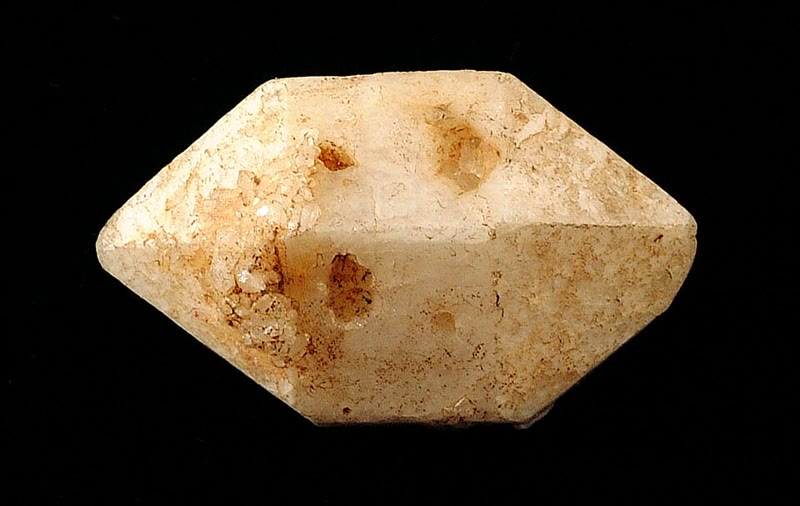
\includegraphics[height=2.75cm]{images/book2/g11-geodil-quartz.jpg}\hfill
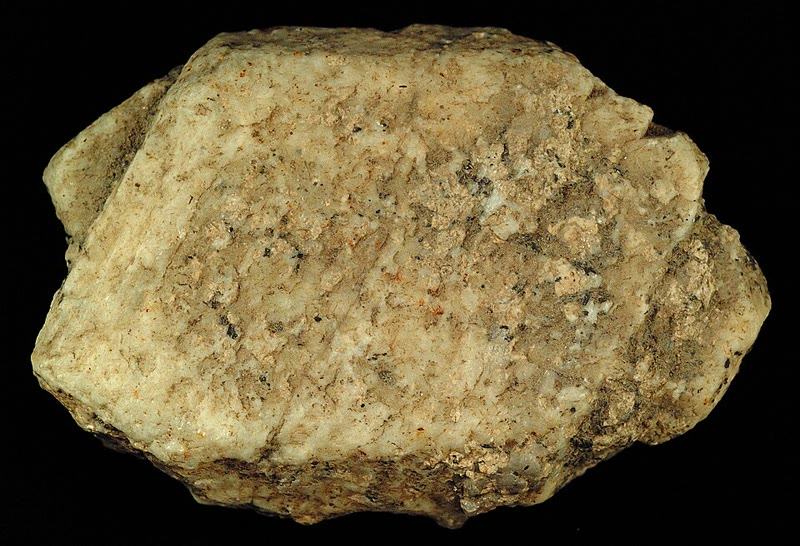
\includegraphics[height=2.75cm]{images/book2/g11-geodil-orthoclase.jpg}\hfill
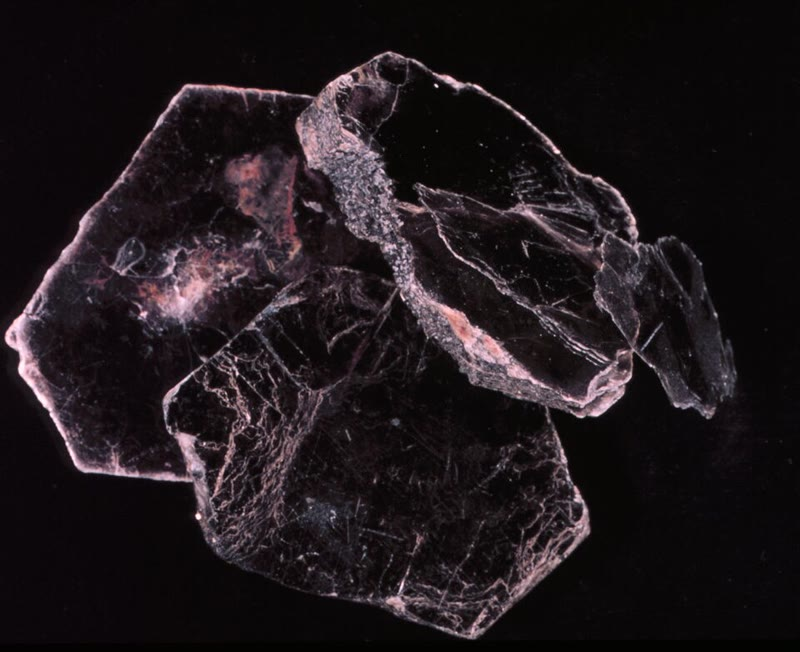
\includegraphics[height=2.75cm]{images/book2/g11-geodil-biotite.jpg}\hfill
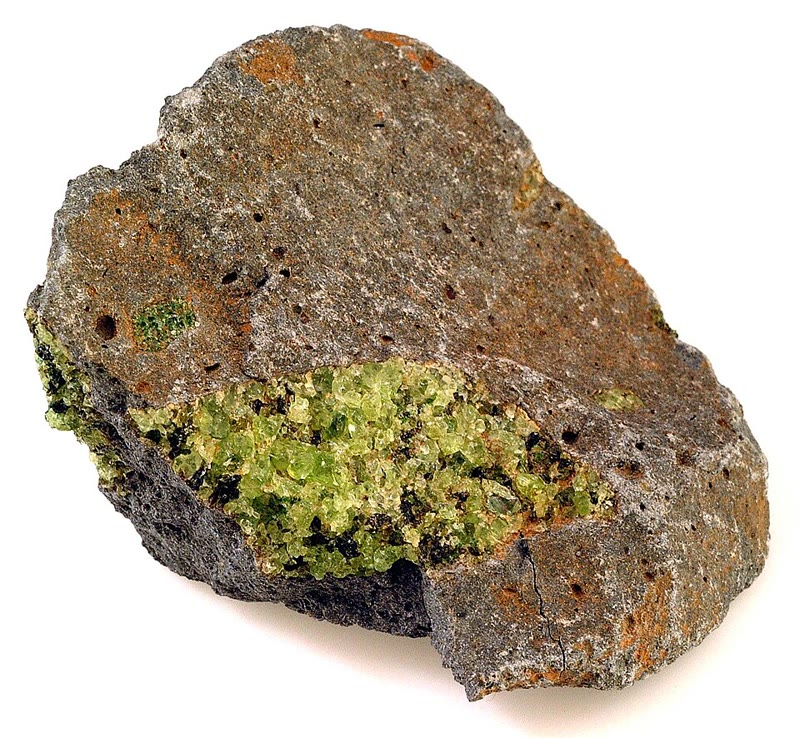
\includegraphics[height=2.75cm]{images/book2/g11-geodil-olivine.jpg}

{\small Cuatro minerales formadores de rocas. De izquierda a derecha: un
cristal de cuarzo, un prisma de seis caras terminado en punta por los dos
extremos, de unos \qty{5}{cm} de largo; un feldespato ortosa, dos cristales
crecidos juntos, de unos \qty{7}{cm}; placas de seis lados de mica biotita, de
unos \qty{6}{cm}, que se separan en láminas finas a lo largo de su única
\omterm{def:g11:minerals:cleavage}{exfoliación}; granos verdes de olivino en un basalto. Fotografías de Shannon
Heinle, Darla Sondrol, Dexter Perkins y Nessa Eull, Geology Digital Image
Library (CC0).}
\end{omfigure}
% ledger: photo:g11-quartz, photo:g11-orthoclase, photo:g11-biotite, photo:g11-olivine

\section{Los silicatos}

\paragraph{Dos elementos forman la corteza.} La composición química de la
corteza continental se conoce gracias a los análisis de muchas rocas,
expresados como porcentajes de óxidos: alrededor del \qty{60.6}{\percent} de
\ce{SiO2}, el \qty{15.9}{\percent} de \ce{Al2O3}, etcétera. A partir de ellos,
y de las masas de los átomos, se obtiene la masa de cada elemento. El oxígeno
forma el \qty{46}{\percent} de la masa de la corteza continental y el silicio
el \qty{28}{\percent}: dos elementos, unas tres cuartas partes de la masa. Con
seis metales ---aluminio, hierro, calcio, magnesio, sodio y potasio--- forman
más del \qty{99}{\percent}.
% ledger: rg14:crust, ciaaw:O, ciaaw:Si, ciaaw:Al, ciaaw:Fe, ciaaw:Ca, ciaaw:Mg, ciaaw:Na, ciaaw:K, ciaaw:Ti, ciaaw:Mn, ciaaw:P
% values (mineral_density.py): bulk_O 46.36, bulk_Si 28.30, O+Si 74.66, eight elements 99.43

\begin{omfigure}
\begin{tikzpicture}
\begin{axis}[omrecord, width=0.82\linewidth, height=5.6cm, ybar, bar width=14pt,
  ymin=0, ymax=55, xtick=data, enlarge x limits=0.06,
  xticklabels from table={figdata/out/grade-11-mineral_density-elements.dat}{symbol},
  ylabel={fracción de la masa (\unit{\percent})},
  nodes near coords, every node near coord/.append style={font=\scriptsize, /pgf/number format/.cd, fixed, precision=1},
  xmajorgrids=false]
% computed in figdata/grade-11/mineral_density.py; ledger: rg14:crust, ciaaw:*
\addplot[fill=omDef!55, draw=omDef] table[x expr=\coordindex, y=frac] {figdata/out/grade-11-mineral_density-elements.dat};
\end{axis}
\end{tikzpicture}

{\small Los elementos de la corteza continental, como fracciones de su masa,
calculadas a partir de su composición media en óxidos (Rudnick y Gao, 2014).
El oxígeno y el silicio forman por sí solos unas tres cuartas partes de la
masa.}
\end{omfigure}

\paragraph{El tetraedro de silicio--oxígeno.} Un átomo de silicio es pequeño,
y a su alrededor caben cuatro átomos de oxígeno, en los vértices de un
tetraedro, una pirámide de cuatro caras triangulares. El grupo contiene un ion
silicio \ce{Si^4+} y cuatro iones óxido \ce{O^2-}: lleva una carga de
$4 - 4 \times 2 = -4$, que otros iones ---u otros tetraedros--- deben
compensar.

\begin{definition}[Silicato; tetraedro de silicio--oxígeno]\label{def:g11:minerals:silicate}
El \emph{tetraedro de silicio--oxígeno}\index{tetraedro de silicio--oxigeno@tetraedro de silicio--oxígeno} es
el grupo \ce{SiO4} formado por un átomo de silicio y los cuatro átomos de
oxígeno que lo rodean, en los vértices de un tetraedro. Un
\emph{silicato}\index{silicato} es un mineral construido con tetraedros de
silicio--oxígeno, aislados o unidos entre sí por vértices compartidos.
\end{definition}
% ledger: tulane:silicates

Los tetraedros se unen compartiendo oxígenos: el vértice de un tetraedro es el
vértice del siguiente. Cuántos vértices comparte cada tetraedro fija la
estructura del \omterm{def:g11:minerals:silicate}{silicato}, y su fórmula.
\begin{itemize}
  \item \emph{Tetraedros aislados}, que no comparten ningún vértice, unidos
        por iones metálicos situados entre ellos: el olivino, \ce{(Mg,Fe)2SiO4}.
  \item \emph{Cadenas sencillas}, en las que cada tetraedro comparte dos
        vértices con sus vecinos: los piroxenos.
  \item \emph{Cadenas dobles}, dos cadenas sencillas unidas lado a lado, con
        tetraedros que comparten alternativamente dos o tres vértices: los
        anfíboles.
  \item \emph{Láminas}, en las que cada tetraedro comparte tres vértices: las
        micas, y los \omterm{def:g10:soil-formation:clay}{minerales de la arcilla} de los suelos (el \cref{ch:g10:soil-formation}).
  \item \emph{Armazones}, en los que cada tetraedro comparte sus cuatro
        vértices, en las tres direcciones del espacio: el cuarzo, \ce{SiO2},
        y ---con aluminio en lugar de parte del silicio--- los feldespatos.
\end{itemize}
% ledger: tulane:silicates

\begin{omfigure}
\begin{tikzpicture}[font=\footnotesize]
  % coordinates generated once by a small script (scratch, not kept): kagome net of side 0.62 cm,
  % a regular tetrahedron in perspective, and a framework piece of five tetrahedra (painter's order)
  % (a) one SiO4 tetrahedron, drawn in perspective; the silicon (black) at its centre
  \fill[omDef!12] (2.300,2.979) -- (1.927,1.372) -- (1.221,0.629) -- (3.752,0.820) -- cycle;
  \draw[densely dashed, omDef!60, line width=0.6pt] (2.300,2.979) -- (1.927,1.372);
  \draw[omDef!70!black, line width=0.6pt] (2.300,2.979) -- (1.221,0.629);
  \draw[omDef!70!black, line width=0.6pt] (2.300,2.979) -- (3.752,0.820);
  \draw[densely dashed, omDef!60, line width=0.6pt] (1.927,1.372) -- (1.221,0.629);
  \draw[densely dashed, omDef!60, line width=0.6pt] (1.927,1.372) -- (3.752,0.820);
  \draw[omDef!70!black, line width=0.6pt] (1.221,0.629) -- (3.752,0.820);
  \draw[black!55, line width=0.4pt] (2.300,1.450) -- (2.300,2.979);
  \draw[black!55, line width=0.4pt] (2.300,1.450) -- (1.927,1.372);
  \draw[black!55, line width=0.4pt] (2.300,1.450) -- (1.221,0.629);
  \draw[black!55, line width=0.4pt] (2.300,1.450) -- (3.752,0.820);
  \fill[black] (2.300,1.450) circle (2.2pt);
  \filldraw[fill=omThm!35, draw=omThm!80!black, line width=0.4pt] (2.300,2.979) circle (4.2pt);
  \filldraw[fill=omThm!35, draw=omThm!80!black, line width=0.4pt] (1.927,1.372) circle (4.2pt);
  \filldraw[fill=omThm!35, draw=omThm!80!black, line width=0.4pt] (1.221,0.629) circle (4.2pt);
  \filldraw[fill=omThm!35, draw=omThm!80!black, line width=0.4pt] (3.752,0.820) circle (4.2pt);
  % coordinates for labels: Si 2.300,1.450; apex 2.300,2.979
  % (b) isolated tetrahedra (olivine)
  \filldraw[fill=omDef!22, draw=omDef!70!black, line width=0.5pt] (6.200,0.900) -- (6.820,0.900) -- (6.510,1.437) -- cycle;
  \fill[black] (6.510,1.079) circle (0.9pt);
  \filldraw[fill=omDef!22, draw=omDef!70!black, line width=0.5pt] (8.370,1.437) -- (8.990,1.437) -- (8.680,1.974) -- cycle;
  \fill[black] (8.680,1.616) circle (0.9pt);
  \filldraw[fill=omDef!22, draw=omDef!70!black, line width=0.5pt] (8.060,1.974) -- (7.750,2.511) -- (8.370,2.511) -- cycle;
  \fill[black] (8.060,2.332) circle (0.9pt);
  \filldraw[fill=omDef!22, draw=omDef!70!black, line width=0.5pt] (8.990,0.363) -- (9.610,0.363) -- (9.300,0.900) -- cycle;
  \fill[black] (9.300,0.542) circle (0.9pt);
  \filldraw[fill=omDef!22, draw=omDef!70!black, line width=0.5pt] (9.920,1.974) -- (9.610,2.511) -- (10.230,2.511) -- cycle;
  \fill[black] (9.920,2.332) circle (0.9pt);
  \filldraw[fill=omThm!35, draw=omThm!80!black, line width=0.4pt] (6.200,0.900) circle (1.9pt);
  \filldraw[fill=omThm!35, draw=omThm!80!black, line width=0.4pt] (6.510,1.437) circle (1.9pt);
  \filldraw[fill=omThm!35, draw=omThm!80!black, line width=0.4pt] (6.820,0.900) circle (1.9pt);
  \filldraw[fill=omThm!35, draw=omThm!80!black, line width=0.4pt] (7.750,2.511) circle (1.9pt);
  \filldraw[fill=omThm!35, draw=omThm!80!black, line width=0.4pt] (8.060,1.974) circle (1.9pt);
  \filldraw[fill=omThm!35, draw=omThm!80!black, line width=0.4pt] (8.370,2.511) circle (1.9pt);
  \filldraw[fill=omThm!35, draw=omThm!80!black, line width=0.4pt] (8.370,1.437) circle (1.9pt);
  \filldraw[fill=omThm!35, draw=omThm!80!black, line width=0.4pt] (8.680,1.974) circle (1.9pt);
  \filldraw[fill=omThm!35, draw=omThm!80!black, line width=0.4pt] (8.990,1.437) circle (1.9pt);
  \filldraw[fill=omThm!35, draw=omThm!80!black, line width=0.4pt] (9.610,2.511) circle (1.9pt);
  \filldraw[fill=omThm!35, draw=omThm!80!black, line width=0.4pt] (8.990,0.363) circle (1.9pt);
  \filldraw[fill=omThm!35, draw=omThm!80!black, line width=0.4pt] (9.300,0.900) circle (1.9pt);
  \filldraw[fill=omThm!35, draw=omThm!80!black, line width=0.4pt] (9.920,1.974) circle (1.9pt);
  \filldraw[fill=omThm!35, draw=omThm!80!black, line width=0.4pt] (10.230,2.511) circle (1.9pt);
  \filldraw[fill=omThm!35, draw=omThm!80!black, line width=0.4pt] (9.610,0.363) circle (1.9pt);
  % (c) single chain (pyroxenes)
  \filldraw[fill=omDef!22, draw=omDef!70!black, line width=0.5pt] (11.400,1.600) -- (12.020,1.600) -- (11.710,2.137) -- cycle;
  \fill[black] (11.710,1.779) circle (0.9pt);
  \filldraw[fill=omDef!22, draw=omDef!70!black, line width=0.5pt] (12.330,1.063) -- (12.020,1.600) -- (12.640,1.600) -- cycle;
  \fill[black] (12.330,1.421) circle (0.9pt);
  \filldraw[fill=omDef!22, draw=omDef!70!black, line width=0.5pt] (12.640,1.600) -- (13.260,1.600) -- (12.950,2.137) -- cycle;
  \fill[black] (12.950,1.779) circle (0.9pt);
  \filldraw[fill=omDef!22, draw=omDef!70!black, line width=0.5pt] (13.570,1.063) -- (13.260,1.600) -- (13.880,1.600) -- cycle;
  \fill[black] (13.570,1.421) circle (0.9pt);
  \filldraw[fill=omDef!22, draw=omDef!70!black, line width=0.5pt] (13.880,1.600) -- (14.500,1.600) -- (14.190,2.137) -- cycle;
  \fill[black] (14.190,1.779) circle (0.9pt);
  \filldraw[fill=omDef!22, draw=omDef!70!black, line width=0.5pt] (14.810,1.063) -- (14.500,1.600) -- (15.120,1.600) -- cycle;
  \fill[black] (14.810,1.421) circle (0.9pt);
  \filldraw[fill=omDef!22, draw=omDef!70!black, line width=0.5pt] (15.120,1.600) -- (15.740,1.600) -- (15.430,2.137) -- cycle;
  \fill[black] (15.430,1.779) circle (0.9pt);
  \filldraw[fill=omThm!35, draw=omThm!80!black, line width=0.4pt] (11.400,1.600) circle (1.9pt);
  \filldraw[fill=omThm!35, draw=omThm!80!black, line width=0.4pt] (11.710,2.137) circle (1.9pt);
  \filldraw[fill=omThm!35, draw=omThm!80!black, line width=0.4pt] (12.020,1.600) circle (1.9pt);
  \filldraw[fill=omThm!35, draw=omThm!80!black, line width=0.4pt] (12.330,1.063) circle (1.9pt);
  \filldraw[fill=omThm!35, draw=omThm!80!black, line width=0.4pt] (12.640,1.600) circle (1.9pt);
  \filldraw[fill=omThm!35, draw=omThm!80!black, line width=0.4pt] (12.950,2.137) circle (1.9pt);
  \filldraw[fill=omThm!35, draw=omThm!80!black, line width=0.4pt] (13.260,1.600) circle (1.9pt);
  \filldraw[fill=omThm!35, draw=omThm!80!black, line width=0.4pt] (13.570,1.063) circle (1.9pt);
  \filldraw[fill=omThm!35, draw=omThm!80!black, line width=0.4pt] (13.880,1.600) circle (1.9pt);
  \filldraw[fill=omThm!35, draw=omThm!80!black, line width=0.4pt] (14.190,2.137) circle (1.9pt);
  \filldraw[fill=omThm!35, draw=omThm!80!black, line width=0.4pt] (14.500,1.600) circle (1.9pt);
  \filldraw[fill=omThm!35, draw=omThm!80!black, line width=0.4pt] (14.810,1.063) circle (1.9pt);
  \filldraw[fill=omThm!35, draw=omThm!80!black, line width=0.4pt] (15.120,1.600) circle (1.9pt);
  \filldraw[fill=omThm!35, draw=omThm!80!black, line width=0.4pt] (15.430,2.137) circle (1.9pt);
  \filldraw[fill=omThm!35, draw=omThm!80!black, line width=0.4pt] (15.740,1.600) circle (1.9pt);
  % (d) double chain (amphiboles)
  \filldraw[fill=omDef!22, draw=omDef!70!black, line width=0.5pt] (0.600,-3.550) -- (1.220,-3.550) -- (0.910,-3.013) -- cycle;
  \fill[black] (0.910,-3.371) circle (0.9pt);
  \filldraw[fill=omDef!22, draw=omDef!70!black, line width=0.5pt] (1.530,-4.087) -- (1.220,-3.550) -- (1.840,-3.550) -- cycle;
  \fill[black] (1.530,-3.729) circle (0.9pt);
  \filldraw[fill=omDef!22, draw=omDef!70!black, line width=0.5pt] (1.840,-3.550) -- (2.460,-3.550) -- (2.150,-3.013) -- cycle;
  \fill[black] (2.150,-3.371) circle (0.9pt);
  \filldraw[fill=omDef!22, draw=omDef!70!black, line width=0.5pt] (2.770,-4.087) -- (2.460,-3.550) -- (3.080,-3.550) -- cycle;
  \fill[black] (2.770,-3.729) circle (0.9pt);
  \filldraw[fill=omDef!22, draw=omDef!70!black, line width=0.5pt] (3.080,-3.550) -- (3.700,-3.550) -- (3.390,-3.013) -- cycle;
  \fill[black] (3.390,-3.371) circle (0.9pt);
  \filldraw[fill=omDef!22, draw=omDef!70!black, line width=0.5pt] (4.010,-4.087) -- (3.700,-3.550) -- (4.320,-3.550) -- cycle;
  \fill[black] (4.010,-3.729) circle (0.9pt);
  \filldraw[fill=omDef!22, draw=omDef!70!black, line width=0.5pt] (4.320,-3.550) -- (4.940,-3.550) -- (4.630,-3.013) -- cycle;
  \fill[black] (4.630,-3.371) circle (0.9pt);
  \filldraw[fill=omDef!22, draw=omDef!70!black, line width=0.5pt] (0.910,-3.013) -- (0.600,-2.476) -- (1.220,-2.476) -- cycle;
  \fill[black] (0.910,-2.655) circle (0.9pt);
  \filldraw[fill=omDef!22, draw=omDef!70!black, line width=0.5pt] (1.220,-2.476) -- (1.840,-2.476) -- (1.530,-1.939) -- cycle;
  \fill[black] (1.530,-2.297) circle (0.9pt);
  \filldraw[fill=omDef!22, draw=omDef!70!black, line width=0.5pt] (2.150,-3.013) -- (1.840,-2.476) -- (2.460,-2.476) -- cycle;
  \fill[black] (2.150,-2.655) circle (0.9pt);
  \filldraw[fill=omDef!22, draw=omDef!70!black, line width=0.5pt] (2.460,-2.476) -- (3.080,-2.476) -- (2.770,-1.939) -- cycle;
  \fill[black] (2.770,-2.297) circle (0.9pt);
  \filldraw[fill=omDef!22, draw=omDef!70!black, line width=0.5pt] (3.390,-3.013) -- (3.080,-2.476) -- (3.700,-2.476) -- cycle;
  \fill[black] (3.390,-2.655) circle (0.9pt);
  \filldraw[fill=omDef!22, draw=omDef!70!black, line width=0.5pt] (3.700,-2.476) -- (4.320,-2.476) -- (4.010,-1.939) -- cycle;
  \fill[black] (4.010,-2.297) circle (0.9pt);
  \filldraw[fill=omDef!22, draw=omDef!70!black, line width=0.5pt] (4.630,-3.013) -- (4.320,-2.476) -- (4.940,-2.476) -- cycle;
  \fill[black] (4.630,-2.655) circle (0.9pt);
  \filldraw[fill=omThm!35, draw=omThm!80!black, line width=0.4pt] (0.600,-2.476) circle (1.9pt);
  \filldraw[fill=omThm!35, draw=omThm!80!black, line width=0.4pt] (0.600,-3.550) circle (1.9pt);
  \filldraw[fill=omThm!35, draw=omThm!80!black, line width=0.4pt] (0.910,-3.013) circle (1.9pt);
  \filldraw[fill=omThm!35, draw=omThm!80!black, line width=0.4pt] (1.220,-2.476) circle (1.9pt);
  \filldraw[fill=omThm!35, draw=omThm!80!black, line width=0.4pt] (1.530,-1.939) circle (1.9pt);
  \filldraw[fill=omThm!35, draw=omThm!80!black, line width=0.4pt] (1.220,-3.550) circle (1.9pt);
  \filldraw[fill=omThm!35, draw=omThm!80!black, line width=0.4pt] (1.840,-2.476) circle (1.9pt);
  \filldraw[fill=omThm!35, draw=omThm!80!black, line width=0.4pt] (1.530,-4.087) circle (1.9pt);
  \filldraw[fill=omThm!35, draw=omThm!80!black, line width=0.4pt] (1.840,-3.550) circle (1.9pt);
  \filldraw[fill=omThm!35, draw=omThm!80!black, line width=0.4pt] (2.150,-3.013) circle (1.9pt);
  \filldraw[fill=omThm!35, draw=omThm!80!black, line width=0.4pt] (2.460,-2.476) circle (1.9pt);
  \filldraw[fill=omThm!35, draw=omThm!80!black, line width=0.4pt] (2.770,-1.939) circle (1.9pt);
  \filldraw[fill=omThm!35, draw=omThm!80!black, line width=0.4pt] (2.460,-3.550) circle (1.9pt);
  \filldraw[fill=omThm!35, draw=omThm!80!black, line width=0.4pt] (3.080,-2.476) circle (1.9pt);
  \filldraw[fill=omThm!35, draw=omThm!80!black, line width=0.4pt] (2.770,-4.087) circle (1.9pt);
  \filldraw[fill=omThm!35, draw=omThm!80!black, line width=0.4pt] (3.080,-3.550) circle (1.9pt);
  \filldraw[fill=omThm!35, draw=omThm!80!black, line width=0.4pt] (3.390,-3.013) circle (1.9pt);
  \filldraw[fill=omThm!35, draw=omThm!80!black, line width=0.4pt] (3.700,-2.476) circle (1.9pt);
  \filldraw[fill=omThm!35, draw=omThm!80!black, line width=0.4pt] (4.010,-1.939) circle (1.9pt);
  \filldraw[fill=omThm!35, draw=omThm!80!black, line width=0.4pt] (3.700,-3.550) circle (1.9pt);
  \filldraw[fill=omThm!35, draw=omThm!80!black, line width=0.4pt] (4.320,-2.476) circle (1.9pt);
  \filldraw[fill=omThm!35, draw=omThm!80!black, line width=0.4pt] (4.010,-4.087) circle (1.9pt);
  \filldraw[fill=omThm!35, draw=omThm!80!black, line width=0.4pt] (4.320,-3.550) circle (1.9pt);
  \filldraw[fill=omThm!35, draw=omThm!80!black, line width=0.4pt] (4.630,-3.013) circle (1.9pt);
  \filldraw[fill=omThm!35, draw=omThm!80!black, line width=0.4pt] (4.940,-2.476) circle (1.9pt);
  \filldraw[fill=omThm!35, draw=omThm!80!black, line width=0.4pt] (4.940,-3.550) circle (1.9pt);
  % (e) sheet (micas)
  \filldraw[fill=omDef!22, draw=omDef!70!black, line width=0.5pt] (5.900,-4.100) -- (6.520,-4.100) -- (6.210,-3.563) -- cycle;
  \fill[black] (6.210,-3.921) circle (0.9pt);
  \filldraw[fill=omDef!22, draw=omDef!70!black, line width=0.5pt] (7.140,-4.100) -- (7.760,-4.100) -- (7.450,-3.563) -- cycle;
  \fill[black] (7.450,-3.921) circle (0.9pt);
  \filldraw[fill=omDef!22, draw=omDef!70!black, line width=0.5pt] (8.380,-4.100) -- (9.000,-4.100) -- (8.690,-3.563) -- cycle;
  \fill[black] (8.690,-3.921) circle (0.9pt);
  \filldraw[fill=omDef!22, draw=omDef!70!black, line width=0.5pt] (9.620,-4.100) -- (10.240,-4.100) -- (9.930,-3.563) -- cycle;
  \fill[black] (9.930,-3.921) circle (0.9pt);
  \filldraw[fill=omDef!22, draw=omDef!70!black, line width=0.5pt] (6.210,-3.563) -- (5.900,-3.026) -- (6.520,-3.026) -- cycle;
  \fill[black] (6.210,-3.205) circle (0.9pt);
  \filldraw[fill=omDef!22, draw=omDef!70!black, line width=0.5pt] (7.450,-3.563) -- (7.140,-3.026) -- (7.760,-3.026) -- cycle;
  \fill[black] (7.450,-3.205) circle (0.9pt);
  \filldraw[fill=omDef!22, draw=omDef!70!black, line width=0.5pt] (8.690,-3.563) -- (8.380,-3.026) -- (9.000,-3.026) -- cycle;
  \fill[black] (8.690,-3.205) circle (0.9pt);
  \filldraw[fill=omDef!22, draw=omDef!70!black, line width=0.5pt] (9.930,-3.563) -- (9.620,-3.026) -- (10.240,-3.026) -- cycle;
  \fill[black] (9.930,-3.205) circle (0.9pt);
  \filldraw[fill=omDef!22, draw=omDef!70!black, line width=0.5pt] (6.520,-3.026) -- (7.140,-3.026) -- (6.830,-2.489) -- cycle;
  \fill[black] (6.830,-2.847) circle (0.9pt);
  \filldraw[fill=omDef!22, draw=omDef!70!black, line width=0.5pt] (7.760,-3.026) -- (8.380,-3.026) -- (8.070,-2.489) -- cycle;
  \fill[black] (8.070,-2.847) circle (0.9pt);
  \filldraw[fill=omDef!22, draw=omDef!70!black, line width=0.5pt] (9.000,-3.026) -- (9.620,-3.026) -- (9.310,-2.489) -- cycle;
  \fill[black] (9.310,-2.847) circle (0.9pt);
  \filldraw[fill=omDef!22, draw=omDef!70!black, line width=0.5pt] (6.830,-2.489) -- (6.520,-1.952) -- (7.140,-1.952) -- cycle;
  \fill[black] (6.830,-2.131) circle (0.9pt);
  \filldraw[fill=omDef!22, draw=omDef!70!black, line width=0.5pt] (8.070,-2.489) -- (7.760,-1.952) -- (8.380,-1.952) -- cycle;
  \fill[black] (8.070,-2.131) circle (0.9pt);
  \filldraw[fill=omDef!22, draw=omDef!70!black, line width=0.5pt] (9.310,-2.489) -- (9.000,-1.952) -- (9.620,-1.952) -- cycle;
  \fill[black] (9.310,-2.131) circle (0.9pt);
  \filldraw[fill=omDef!22, draw=omDef!70!black, line width=0.5pt] (5.900,-1.952) -- (6.520,-1.952) -- (6.210,-1.415) -- cycle;
  \fill[black] (6.210,-1.773) circle (0.9pt);
  \filldraw[fill=omDef!22, draw=omDef!70!black, line width=0.5pt] (7.140,-1.952) -- (7.760,-1.952) -- (7.450,-1.415) -- cycle;
  \fill[black] (7.450,-1.773) circle (0.9pt);
  \filldraw[fill=omDef!22, draw=omDef!70!black, line width=0.5pt] (8.380,-1.952) -- (9.000,-1.952) -- (8.690,-1.415) -- cycle;
  \fill[black] (8.690,-1.773) circle (0.9pt);
  \filldraw[fill=omDef!22, draw=omDef!70!black, line width=0.5pt] (9.620,-1.952) -- (10.240,-1.952) -- (9.930,-1.415) -- cycle;
  \fill[black] (9.930,-1.773) circle (0.9pt);
  \filldraw[fill=omThm!35, draw=omThm!80!black, line width=0.4pt] (5.900,-1.952) circle (1.9pt);
  \filldraw[fill=omThm!35, draw=omThm!80!black, line width=0.4pt] (6.210,-1.415) circle (1.9pt);
  \filldraw[fill=omThm!35, draw=omThm!80!black, line width=0.4pt] (5.900,-3.026) circle (1.9pt);
  \filldraw[fill=omThm!35, draw=omThm!80!black, line width=0.4pt] (6.520,-1.952) circle (1.9pt);
  \filldraw[fill=omThm!35, draw=omThm!80!black, line width=0.4pt] (5.900,-4.100) circle (1.9pt);
  \filldraw[fill=omThm!35, draw=omThm!80!black, line width=0.4pt] (6.210,-3.563) circle (1.9pt);
  \filldraw[fill=omThm!35, draw=omThm!80!black, line width=0.4pt] (6.520,-3.026) circle (1.9pt);
  \filldraw[fill=omThm!35, draw=omThm!80!black, line width=0.4pt] (6.830,-2.489) circle (1.9pt);
  \filldraw[fill=omThm!35, draw=omThm!80!black, line width=0.4pt] (7.140,-1.952) circle (1.9pt);
  \filldraw[fill=omThm!35, draw=omThm!80!black, line width=0.4pt] (7.450,-1.415) circle (1.9pt);
  \filldraw[fill=omThm!35, draw=omThm!80!black, line width=0.4pt] (6.520,-4.100) circle (1.9pt);
  \filldraw[fill=omThm!35, draw=omThm!80!black, line width=0.4pt] (7.140,-3.026) circle (1.9pt);
  \filldraw[fill=omThm!35, draw=omThm!80!black, line width=0.4pt] (7.760,-1.952) circle (1.9pt);
  \filldraw[fill=omThm!35, draw=omThm!80!black, line width=0.4pt] (7.140,-4.100) circle (1.9pt);
  \filldraw[fill=omThm!35, draw=omThm!80!black, line width=0.4pt] (7.450,-3.563) circle (1.9pt);
  \filldraw[fill=omThm!35, draw=omThm!80!black, line width=0.4pt] (7.760,-3.026) circle (1.9pt);
  \filldraw[fill=omThm!35, draw=omThm!80!black, line width=0.4pt] (8.070,-2.489) circle (1.9pt);
  \filldraw[fill=omThm!35, draw=omThm!80!black, line width=0.4pt] (8.380,-1.952) circle (1.9pt);
  \filldraw[fill=omThm!35, draw=omThm!80!black, line width=0.4pt] (8.690,-1.415) circle (1.9pt);
  \filldraw[fill=omThm!35, draw=omThm!80!black, line width=0.4pt] (7.760,-4.100) circle (1.9pt);
  \filldraw[fill=omThm!35, draw=omThm!80!black, line width=0.4pt] (8.380,-3.026) circle (1.9pt);
  \filldraw[fill=omThm!35, draw=omThm!80!black, line width=0.4pt] (9.000,-1.952) circle (1.9pt);
  \filldraw[fill=omThm!35, draw=omThm!80!black, line width=0.4pt] (8.380,-4.100) circle (1.9pt);
  \filldraw[fill=omThm!35, draw=omThm!80!black, line width=0.4pt] (8.690,-3.563) circle (1.9pt);
  \filldraw[fill=omThm!35, draw=omThm!80!black, line width=0.4pt] (9.000,-3.026) circle (1.9pt);
  \filldraw[fill=omThm!35, draw=omThm!80!black, line width=0.4pt] (9.310,-2.489) circle (1.9pt);
  \filldraw[fill=omThm!35, draw=omThm!80!black, line width=0.4pt] (9.620,-1.952) circle (1.9pt);
  \filldraw[fill=omThm!35, draw=omThm!80!black, line width=0.4pt] (9.930,-1.415) circle (1.9pt);
  \filldraw[fill=omThm!35, draw=omThm!80!black, line width=0.4pt] (9.000,-4.100) circle (1.9pt);
  \filldraw[fill=omThm!35, draw=omThm!80!black, line width=0.4pt] (9.620,-3.026) circle (1.9pt);
  \filldraw[fill=omThm!35, draw=omThm!80!black, line width=0.4pt] (10.240,-1.952) circle (1.9pt);
  \filldraw[fill=omThm!35, draw=omThm!80!black, line width=0.4pt] (9.620,-4.100) circle (1.9pt);
  \filldraw[fill=omThm!35, draw=omThm!80!black, line width=0.4pt] (9.930,-3.563) circle (1.9pt);
  \filldraw[fill=omThm!35, draw=omThm!80!black, line width=0.4pt] (10.240,-3.026) circle (1.9pt);
  \filldraw[fill=omThm!35, draw=omThm!80!black, line width=0.4pt] (10.240,-4.100) circle (1.9pt);
  % (f) framework: a tetrahedron sharing all four corners
  \filldraw[fill=omThm!35, draw=omThm!80!black, line width=0.4pt] (12.990,-1.963) circle (2.1pt);
  \filldraw[fill=omThm!35, draw=omThm!80!black, line width=0.4pt] (12.896,-3.062) circle (2.1pt);
  \filldraw[fill=omDef!14, draw=omDef!70!black, line width=0.45pt, fill opacity=0.85] (12.896,-3.062) -- (12.990,-1.963) -- (12.299,-2.380) -- cycle;
  \filldraw[fill=omThm!35, draw=omThm!80!black, line width=0.4pt] (15.186,-2.119) circle (2.1pt);
  \filldraw[fill=omDef!14, draw=omDef!70!black, line width=0.45pt, fill opacity=0.85] (12.896,-3.062) -- (13.398,-2.458) -- (12.990,-1.963) -- cycle;
  \filldraw[fill=omThm!35, draw=omThm!80!black, line width=0.4pt] (15.092,-3.219) circle (2.1pt);
  \fill[black] (12.896,-2.466) circle (1.1pt);
  \filldraw[fill=omDef!34, draw=omDef!70!black, line width=0.45pt, fill opacity=0.85] (13.398,-2.458) -- (12.990,-1.963) -- (12.299,-2.380) -- cycle;
  \filldraw[fill=omDef!14, draw=omDef!70!black, line width=0.45pt, fill opacity=0.85] (15.092,-3.219) -- (15.186,-2.119) -- (14.496,-2.536) -- cycle;
  \filldraw[fill=omDef!25, draw=omDef!70!black, line width=0.45pt, fill opacity=0.85] (12.896,-3.062) -- (12.299,-2.380) -- (13.398,-2.458) -- cycle;
  \filldraw[fill=omDef!14, draw=omDef!70!black, line width=0.45pt, fill opacity=0.85] (15.092,-3.219) -- (15.595,-2.614) -- (15.186,-2.119) -- cycle;
  \fill[black] (15.092,-2.622) circle (1.1pt);
  \filldraw[fill=omThm!35, draw=omThm!80!black, line width=0.4pt] (12.299,-2.380) circle (2.1pt);
  \filldraw[fill=omDef!34, draw=omDef!70!black, line width=0.45pt, fill opacity=0.85] (15.595,-2.614) -- (15.186,-2.119) -- (14.496,-2.536) -- cycle;
  \filldraw[fill=omDef!25, draw=omDef!70!black, line width=0.45pt, fill opacity=0.85] (15.092,-3.219) -- (14.496,-2.536) -- (15.595,-2.614) -- cycle;
  \filldraw[fill=omThm!35, draw=omThm!80!black, line width=0.4pt] (13.398,-2.458) circle (2.1pt);
  \filldraw[fill=omThm!35, draw=omThm!80!black, line width=0.4pt] (14.496,-2.536) circle (2.1pt);
  \filldraw[fill=omDef!14, draw=omDef!70!black, line width=0.45pt, fill opacity=0.85] (13.900,-1.853) -- (14.496,-2.536) -- (13.398,-2.458) -- cycle;
  \filldraw[fill=omThm!35, draw=omThm!80!black, line width=0.4pt] (15.595,-2.614) circle (2.1pt);
  \filldraw[fill=omDef!14, draw=omDef!70!black, line width=0.45pt, fill opacity=0.85] (13.398,-2.458) -- (13.806,-2.953) -- (14.496,-2.536) -- cycle;
  \fill[black] (13.900,-2.450) circle (1.1pt);
  \filldraw[fill=omDef!22, draw=omDef!70!black, line width=0.45pt, fill opacity=0.85] (13.900,-1.853) -- (13.398,-2.458) -- (13.806,-2.953) -- cycle;
  \filldraw[fill=omDef!37, draw=omDef!70!black, line width=0.45pt, fill opacity=0.85] (13.900,-1.853) -- (13.806,-2.953) -- (14.496,-2.536) -- cycle;
  \filldraw[fill=omThm!35, draw=omThm!80!black, line width=0.4pt] (13.994,-0.754) circle (2.1pt);
  \filldraw[fill=omThm!35, draw=omThm!80!black, line width=0.4pt] (13.900,-1.853) circle (2.1pt);
  \filldraw[fill=omThm!35, draw=omThm!80!black, line width=0.4pt] (13.806,-2.953) circle (2.1pt);
  \filldraw[fill=omDef!14, draw=omDef!70!black, line width=0.45pt, fill opacity=0.85] (13.900,-1.853) -- (13.994,-0.754) -- (13.304,-1.171) -- cycle;
  \filldraw[fill=omDef!14, draw=omDef!70!black, line width=0.45pt, fill opacity=0.85] (13.900,-1.853) -- (14.402,-1.249) -- (13.994,-0.754) -- cycle;
  \filldraw[fill=omThm!35, draw=omThm!80!black, line width=0.4pt] (13.712,-4.053) circle (2.1pt);
  \fill[black] (13.900,-1.256) circle (1.1pt);
  \filldraw[fill=omDef!14, draw=omDef!70!black, line width=0.45pt, fill opacity=0.85] (13.712,-4.053) -- (13.806,-2.953) -- (13.116,-3.370) -- cycle;
  \filldraw[fill=omDef!34, draw=omDef!70!black, line width=0.45pt, fill opacity=0.85] (14.402,-1.249) -- (13.994,-0.754) -- (13.304,-1.171) -- cycle;
  \filldraw[fill=omDef!14, draw=omDef!70!black, line width=0.45pt, fill opacity=0.85] (13.712,-4.053) -- (14.214,-3.448) -- (13.806,-2.953) -- cycle;
  \filldraw[fill=omDef!25, draw=omDef!70!black, line width=0.45pt, fill opacity=0.85] (13.900,-1.853) -- (13.304,-1.171) -- (14.402,-1.249) -- cycle;
  \fill[black] (13.712,-3.456) circle (1.1pt);
  \filldraw[fill=omThm!35, draw=omThm!80!black, line width=0.4pt] (13.304,-1.171) circle (2.1pt);
  \filldraw[fill=omDef!34, draw=omDef!70!black, line width=0.45pt, fill opacity=0.85] (14.214,-3.448) -- (13.806,-2.953) -- (13.116,-3.370) -- cycle;
  \filldraw[fill=omDef!25, draw=omDef!70!black, line width=0.45pt, fill opacity=0.85] (13.712,-4.053) -- (13.116,-3.370) -- (14.214,-3.448) -- cycle;
  \filldraw[fill=omThm!35, draw=omThm!80!black, line width=0.4pt] (14.402,-1.249) circle (2.1pt);
  \filldraw[fill=omThm!35, draw=omThm!80!black, line width=0.4pt] (13.116,-3.370) circle (2.1pt);
  \filldraw[fill=omThm!35, draw=omThm!80!black, line width=0.4pt] (14.214,-3.448) circle (2.1pt);
  % labels
  \draw[black!60] (2.30,2.98) -- (3.35,3.25); \node[anchor=west] at (3.35,3.25) {oxígeno};
  \draw[black!60] (2.30,1.45) -- (3.55,2.15); \node[anchor=west] at (3.55,2.15) {silicio};
  \node[align=center] at (2.3,-0.15) {(a) un tetraedro, \ce{SiO4}};
  \node[align=center] at (8.2,-0.15) {(b) tetraedros aislados:\\olivino};
  \node[align=center] at (13.5,-0.15) {(c) cadena sencilla:\\piroxenos};
  \node[align=center] at (2.75,-4.85) {(d) cadena doble:\\anfíboles};
  \node[align=center] at (8.1,-4.85) {(e) lámina:\\micas};
  \node[align=center] at (13.9,-4.85) {(f) armazón:\\cuarzo, feldespatos};
\end{tikzpicture}

{\small (a) El \omterm{def:g11:minerals:silicate}{tetraedro de silicio--oxígeno}: un átomo de silicio (negro) y
cuatro átomos de oxígeno (rosa) en los vértices de un tetraedro. (b)--(e)
Tetraedros vistos desde arriba, cada uno como un triángulo: los círculos son
los oxígenos de su base, y el punto, el silicio, bajo el cuarto oxígeno; dos
triángulos que se tocan en un vértice comparten ese oxígeno. (f) En un
armazón se comparten todos los vértices, en tres dimensiones: aquí, un
tetraedro y sus cuatro vecinos. Dibujos, no a escala.}
\end{omfigure}
% ledger: tulane:silicates

\begin{proposition}[Contar los oxígenos]\label{prop:g11:minerals:sharing}
En un \omterm{def:g11:minerals:silicate}{silicato} en el que cada tetraedro comparte $n$ de sus vértices con otros
tetraedros, hay $4 - n/2$ átomos de oxígeno por cada átomo de silicio. Los
tetraedros aislados dan \ce{SiO4}, las cadenas sencillas \ce{SiO3}, las
láminas \ce{Si2O5} y los armazones \ce{SiO2}.
\end{proposition}

\begin{proof}
Cada tetraedro tiene un silicio y cuatro vértices. Un vértice no compartido
pertenece solo a ese tetraedro y cuenta como un oxígeno; un vértice compartido
pertenece a dos tetraedros y cuenta como medio oxígeno en cada uno. Con
$n$ vértices compartidos, un tetraedro posee $(4 - n) + n/2 = 4 - n/2$ oxígenos.
Para $n = 0$, $2$, $3$ y $4$ esto da $4$, $3$, $5/2$ y $2$ oxígenos
por silicio: \ce{SiO4}, \ce{SiO3}, \ce{Si2O5} y \ce{SiO2}.
\end{proof}

Las fórmulas de los minerales lo confirman. El piroxeno augita contiene
\ce{(Si,Al)2O6}, es decir, dos veces \ce{SiO3}, y la mica biotita \ce{AlSi3O10},
cuatro tetraedros para diez oxígenos, dos veces \ce{Si2O5}; en un feldespato,
cuatro tetraedros tienen ocho oxígenos, cuatro veces \ce{SiO2}, exactamente
como en el cuarzo. Las cargas, sin embargo, son distintas. El cuarzo es
neutro: en un armazón todos los oxígenos se comparten, y las cargas del
silicio y del oxígeno se compensan. En las demás estructuras, los oxígenos no
compartidos llevan cargas negativas sobrantes, compensadas por iones
metálicos ---magnesio y hierro en el olivino, potasio en la ortosa, donde un
ion aluminio \ce{Al^3+} en lugar de un ion silicio \ce{Si^4+} deja una carga
por compensar.
% ledger: wm:densities (formulas)

\begin{definition}[Silicatos formadores de rocas]\label{def:g11:minerals:rock-forming}
Los \emph{silicatos formadores de rocas}\index{silicatos formadores de rocas} son
los seis grupos de minerales silicatados que forman la mayoría de las rocas
ígneas y metamórficas comunes: el olivino, los piroxenos, los anfíboles, las
micas, los feldespatos y el cuarzo. Los feldespatos son de dos tipos: el
\emph{feldespato potásico}, como la ortosa, y la \emph{plagioclasa}, una serie
de feldespatos que contienen sodio y calcio.
\end{definition}
% ledger: tulane:silicates, wm:densities

\begin{center}
\small
\renewcommand{\arraystretch}{1.25}
\begin{tabular}{|l|l|l|c|}
\hline
\textbf{grupo (ejemplo)} & \textbf{estructura} & \textbf{fórmula} & \textbf{densidad} \\
 & & & (\unit{g/cm^3}) \\
\hline
olivino & tetraedros aislados & \ce{(Mg,Fe)2SiO4} & 3.32 \\
piroxeno (augita) & cadenas sencillas & \ce{(Ca,Na)(Mg,Fe,Al,Ti)(Si,Al)2O6} & 3.4 \\
anfíbol (hornblenda) & cadenas dobles & \ce{Ca2[Mg4(Al,Fe)]Si7AlO22(OH)2} & 3.23 \\
mica (biotita) & láminas & \ce{K(Mg,Fe)3AlSi3O10(OH,F)2} & 3.09 \\
mica (moscovita) & láminas & \ce{KAl2(Si3Al)O10(OH,F)2} & 2.82 \\
feldespato potásico (ortosa) & armazón & \ce{KAlSi3O8} & 2.56 \\
plagioclasa (oligoclasa) & armazón & \ce{(Na,Ca)(Si,Al)4O8} & 2.65 \\
cuarzo & armazón & \ce{SiO2} & 2.62 \\
\hline
\end{tabular}

\smallskip
{\footnotesize Los \omterm{def:g11:minerals:rock-forming}{silicatos formadores de rocas}. Fórmulas y densidades medias
de webmineral.com; una coma entre dos elementos entre paréntesis indica que
cualquiera de los dos puede ocupar ese lugar en el cristal.}
\end{center}
% ledger: wm:densities, tulane:silicates

La tabla contiene una regla que recorre el resto de este libro. Los minerales
de tetraedros aislados y de cadenas, ricos en hierro y magnesio, son los más
densos, por encima de \qty{3.2}{g/cm^3}; los armazones, formados por silicio,
aluminio, sodio, potasio y calcio, son los más ligeros, de unos
\qty{2.6}{g/cm^3}. Las micas quedan en medio. El olivino y el piroxeno forman
la \omterm{def:g11:ocean-ridges:peridotite}{peridotita} del manto; los feldespatos y el cuarzo, el granito de los
continentes: la roca ligera flota sobre la densa.
% ledger: wm:densities

\section{Los minerales forman las rocas}

Una roca se describe primero por sus minerales y sus proporciones. Tres rocas
vistas en capítulos anteriores muestran la variedad:
\begin{itemize}
  \item el \emph{granito}: cuarzo, feldespato potásico y plagioclasa, con un
        poco de biotita o de moscovita ---la roca de los continentes---;
  \item el \emph{basalto} y el \emph{\omterm{def:g11:ocean-ridges:gabbro}{gabro}}: plagioclasa y piroxeno, a menudo
        con olivino ---las rocas de la \omterm{def:g11:ocean-ridges:oceanic-lithosphere}{corteza oceánica}, el primero de grano
        fino, el segundo de grano grueso--- (el \cref{ch:g11:igneous-rocks});
  \item la \emph{\omterm{def:g11:ocean-ridges:peridotite}{peridotita}}: sobre todo olivino, con piroxeno ---la roca del
        manto.
\end{itemize}
% ledger: nps:granite-minerals, photo:g11-basalt-thin-section, photo:g11-olivine

\begin{omfigure}
\begin{tikzpicture}
\begin{axis}[omrecord, width=0.8\linewidth, height=6.4cm, xbar, bar width=8pt,
  xmin=2.4, xmax=3.5, ymin=-0.7, ymax=8.7, ytick={0,...,8},
  yticklabels={ortosa, cuarzo, oligoclasa, labradorita, moscovita, biotita, hornblenda, olivino, augita},
  xlabel={densidad (\unit{g/cm^3})}, ymajorgrids=false, clip=false]
% computed in figdata/grade-11/mineral_density.py (density_order); ledger: wm:densities
\addplot[fill=omDef!45, draw=omDef] table[x=rho, y=idx] {figdata/out/grade-11-mineral_density-densities.dat};
\draw[omProp, line width=1pt, dashed] (axis cs:2.6427,-0.7) -- (axis cs:2.6427,8.7) node[above, text height=1.6ex, text depth=0.3ex, font=\scriptsize, text=omProp!80!black] {granito};
\draw[omThm, line width=1pt, dashed] (axis cs:3.0015,-0.7) -- (axis cs:3.0015,8.7) node[above, text height=1.6ex, text depth=0.3ex, font=\scriptsize, text=omThm] {basalto};
\draw[black!70, line width=1pt, dashed] (axis cs:3.34,-0.7) -- (axis cs:3.34,8.7) node[above, font=\scriptsize] {peridotita};
\end{axis}
\end{tikzpicture}

{\small Las densidades medias de nueve minerales formadores de rocas
(webmineral.com), y las densidades de las tres rocas de ejemplo de esta
sección calculadas con la proposición siguiente (líneas discontinuas): un
granito de cuarzo, feldespatos y micas, un basalto de plagioclasa, piroxeno y
algo de olivino, y una \omterm{def:g11:ocean-ridges:peridotite}{peridotita} de olivino y piroxeno.}
\end{omfigure}
% values (mineral_density.py): rho_granite 2.6427, rho_basalt 3.0015, rho_peridotite 3.34

La densidad de una roca se deduce de sus minerales. Imagina un bloque de roca
de volumen $V$, del que una fracción $\phi_1$ está formada por un primer
mineral, $\phi_2$ por un segundo, y así sucesivamente.

\begin{proposition}[La densidad de una roca a partir de sus minerales]\label{prop:g11:minerals:density}
Una roca sin poros, formada por minerales de densidades $\rho_1, \rho_2, \dots,
\rho_k$ que ocupan las fracciones $\phi_1, \phi_2, \dots, \phi_k$ de su volumen
($\phi_1 + \dots + \phi_k = 1$), tiene la densidad
\[
  \rho = \phi_1 \rho_1 + \phi_2 \rho_2 + \dots + \phi_k \rho_k ,
\]
la media de las densidades de sus minerales, ponderada por sus fracciones de
volumen.
\end{proposition}

\begin{proof}
En un volumen $V$ de roca, el mineral $i$ ocupa el volumen $\phi_i V$ y tiene
la masa $\rho_i \phi_i V$. Sin poros, la masa de la roca es la suma de estas
masas, $m = (\phi_1 \rho_1 + \dots + \phi_k \rho_k)\,V$, y su densidad es
$m/V$.
\end{proof}

¿Cómo se miden las fracciones de volumen? Sobre una cara plana cortada de la
roca, o sobre una \omterm{def:g11:minerals:thin-section}{lámina delgada} (sección siguiente), se dispone una
cuadrícula regular de puntos, y en cada punto se anota el mineral que hay
debajo. Cuando los granos están repartidos sin orden, la fracción de puntos
que caen sobre un mineral estima la fracción de la superficie que cubre, y esa
es también la fracción del volumen que ocupa: una lámina fina es una muestra
representativa del bloque entero. Es un \emph{recuento de puntos}.

\begin{example}[Un granito ligero de cuarzo y feldespato potásico]
Un recuento de puntos da un \qty{35}{\percent} de cuarzo (\qty{2.62}{g/cm^3}),
un \qty{50}{\percent} de ortosa (\qty{2.56}{g/cm^3}) y un \qty{15}{\percent}
de oligoclasa (\qty{2.65}{g/cm^3}). La densidad de la roca es
\[
  \rho = 0.35 \times 2.62 + 0.50 \times 2.56 + 0.15 \times 2.65
       = 0.917 + 1.280 + 0.398 \approx \qty{2.59}{g/cm^3}.
\]
Las medidas confirman este orden de magnitud: de \num{6454} muestras de roca
pesadas en unos doscientos cuerpos de roca granítica de Sierra Nevada, en
California, la media es de \qty{2.69}{g/cm^3}, y los granitos más ricos en
sílice y potasio, como este, quedan por debajo de \qty{2.6}{g/cm^3}.
\end{example}
% ledger: wm:densities, usgs91:sierra

\section{Las láminas delgadas}

Una lupa muestra granos de un milímetro. Para ver granos más finos, e
identificarlos con certeza, los geólogos observan las rocas al microscopio
---no su superficie, sino a través de ellas.

\begin{definition}[Lámina delgada; microscopio de polarización]\label{def:g11:minerals:thin-section}
Una \emph{lámina delgada}\index{lamina delgada@lámina delgada} es una lámina de roca
desgastada hasta un espesor de \qty{0.03}{mm} y montada sobre un
portaobjetos de vidrio: con ese espesor, la luz atraviesa la mayoría de los
minerales. Un \emph{microscopio de
polarización}\index{microscopio de polarizacion@microscopio de polarización} es un microscopio equipado
con dos filtros polarizadores, uno bajo el portaobjetos y otro encima. La
lámina se observa con \emph{luz polarizada plana} con el filtro inferior solo,
y entre \emph{polarizadores cruzados} cuando se añade el filtro superior con
su dirección perpendicular a la del inferior.
\end{definition}
% ledger: tulane:thin-section

\begin{omfigure}
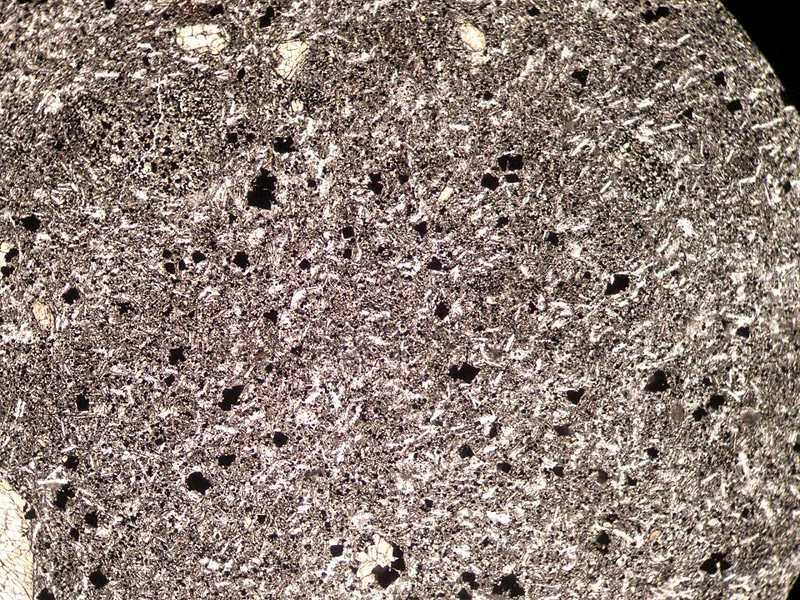
\includegraphics[height=3.6cm]{images/book2/g11-chmee2-basalt-ppl.jpg}\hfill
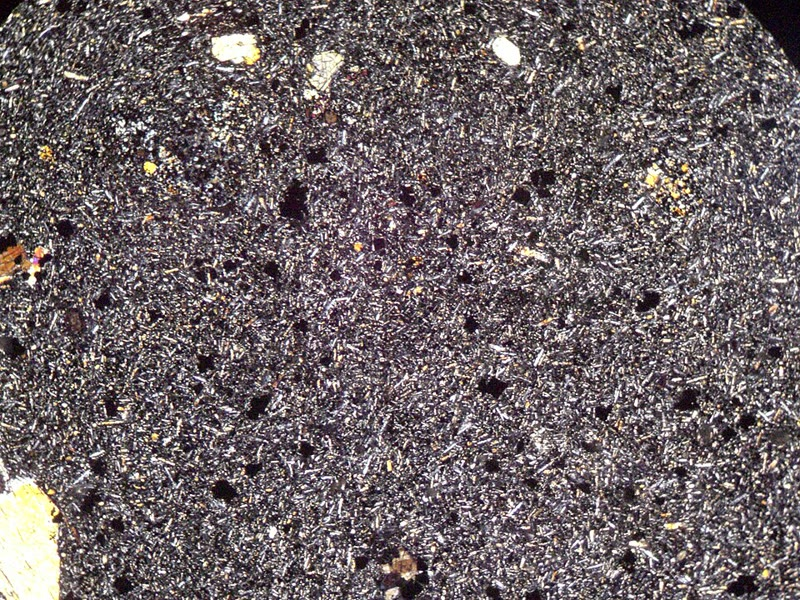
\includegraphics[height=3.6cm]{images/book2/g11-chmee2-basalt-xpl.jpg}\hfill
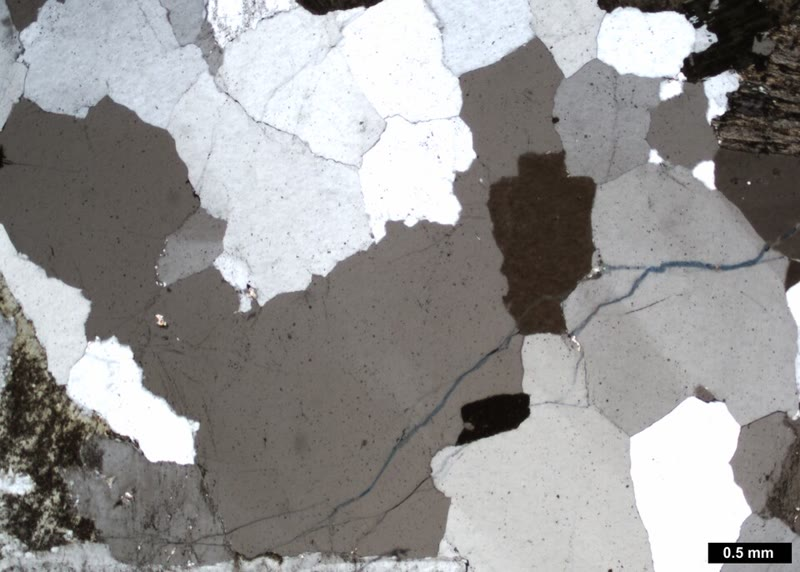
\includegraphics[height=3.6cm]{images/book2/g11-rygel-granite-xpl.jpg}

{\small A la izquierda y en el centro: el mismo basalto en \omterm{def:g11:minerals:thin-section}{lámina delgada}, con
luz polarizada plana y entre polarizadores cruzados. La roca es de grano fino:
pequeños cristales alargados, sobre todo de plagioclasa, y puntos negros que
no dejan pasar la luz en ninguna de las dos vistas; entre polarizadores
cruzados, los cristales se iluminan en grises y en colores. Fotografías de
Chmee2 (CC~BY-SA~3.0). A la derecha: cristales de cuarzo en un granito, entre
polarizadores cruzados, cada uno con su propio tono de gris (la barra de
escala mide \qty{0.5}{mm}). Fotografía de Michael C.~Rygel (CC~BY-SA~3.0).}
\end{omfigure}
% ledger: photo:g11-basalt-thin-section, photo:g11-granite-thin-section

Con luz polarizada plana, una \omterm{def:g11:minerals:thin-section}{lámina delgada} parece una vidriera: la mayoría
de los minerales son casi incoloros, algunos están teñidos, y los contornos de
los granos, sus exfoliaciones y sus \omterm{def:g11:minerals:habit}{hábitos} se ven con nitidez. Entre
polarizadores cruzados, los filtros, colocados uno perpendicular al otro, no
dejarían pasar ninguna luz por sí solos; la mayoría de los minerales alteran
la luz que los atraviesa, y aparecen en tonos de gris o en colores vivos, que
cambian al girar el portaobjetos. Dos granos del mismo mineral pueden verse
distintos, porque cada uno está cortado en su propia dirección: los granos de
cuarzo del granito de arriba son todos de cuarzo, con tonos distintos. Los
colores, cómo cambian y lo que revelan de cada mineral son materia del primer
año de universidad; aquí, la \omterm{def:g11:minerals:thin-section}{lámina delgada} es una imagen de la roca, en la
que cada grano puede verse, nombrarse y contarse.

\section{Ejercicios}

\begin{exercise}[$\star$]\label{exo:g11:minerals:1}
Define la \omterm{def:g11:minerals:cleavage}{exfoliación} y la \omterm{def:g11:minerals:cleavage}{fractura}. ¿Cuál de las dos muestra el cuarzo, y qué
aspecto tienen sus superficies rotas? ¿Cuántas exfoliaciones tiene una mica?
\end{exercise}

\begin{exercise}[$\star$]\label{exo:g11:minerals:2}
¿Por qué el color es una mala guía para identificar el cuarzo, pero bastante
buena para el olivino? Da dos propiedades más fiables que el color.
\end{exercise}

\begin{exercise}[$\star$]\label{exo:g11:minerals:3}
Asocia cada descripción a un mineral entre cuarzo, ortosa, biotita y olivino:
(1) granos verdes en un basalto; (2) escamas negras que se separan en láminas
finas; (3) granos rosados y macizos con dos planos de rotura lisos, que raya un
clavo de acero; (4) granos grises y vítreos con roturas curvas, que el clavo
no raya.
\end{exercise}

\begin{exercise}[$\star$]\label{exo:g11:minerals:4}
(1) ¿Cuántos átomos contiene un \omterm{def:g11:minerals:silicate}{tetraedro de silicio--oxígeno}, y dónde están?
(2) Con las cargas de los iones \ce{Si^4+} y \ce{O^2-}, halla la carga del
grupo \ce{SiO4}.
\end{exercise}

\begin{exercise}[$\star$]\label{exo:g11:minerals:5}
Nombra los seis grupos de \omterm{def:g11:minerals:rock-forming}{silicatos formadores de rocas} e indica, para cada
uno, cómo se unen sus tetraedros.
\end{exercise}

\begin{exercise}[$\star\star$]\label{exo:g11:minerals:6}
Las masas atómicas del silicio y del oxígeno son \qty{28.085}{g/mol} y
\qty{15.999}{g/mol}. (1) Calcula la fracción de oxígeno en la masa del cuarzo,
\ce{SiO2}. (2) Haz lo mismo para la forsterita, el olivino de magnesio
\ce{Mg2SiO4} (magnesio: \qty{24.305}{g/mol}). (3) Compáralo con la fracción
de oxígeno en la corteza continental, alrededor del \qty{46}{\percent}.
\end{exercise}

\begin{exercise}[$\star\star$]\label{exo:g11:minerals:7}
Un grano blanco de un granito raya una placa de vidrio (alrededor de 5.5),
pero lo raya un clavo de acero (alrededor de 6.5); se rompe según planos lisos
en dos direcciones. Un segundo grano, gris, no lo raya el clavo y se rompe
según superficies curvas. Identifica los dos, dando las razones.
\end{exercise}

\begin{exercise}[$\star\star$]\label{exo:g11:minerals:8}
En el piroxeno augita, cada tetraedro comparte dos vértices. (1) Con la
proposición sobre el recuento de los oxígenos, ¿cuántos oxígenos hay por cada
silicio? (2) Comprueba que la parte \ce{(Si,Al)2O6} de la fórmula de la augita
concuerda.
\end{exercise}

\begin{exercise}[$\star\star$]\label{exo:g11:minerals:9}
Un basalto está formado, en volumen, por un \qty{55}{\percent} de
labradorita (\qty{2.69}{g/cm^3}), un \qty{35}{\percent} de augita
(\qty{3.4}{g/cm^3}) y un \qty{10}{\percent} de olivino (\qty{3.32}{g/cm^3}).
Calcula su densidad y, luego, la masa de un cubo de este basalto de
\qty{10}{cm} de arista.
\end{exercise}

\begin{exercise}[$\star\star$]\label{exo:g11:minerals:10}
Una \omterm{def:g11:ocean-ridges:peridotite}{peridotita} del manto está formada por un \qty{75}{\percent} de olivino
(\qty{3.32}{g/cm^3}) y un \qty{25}{\percent} de augita (\qty{3.4}{g/cm^3}).
(1) Calcula su densidad. (2) ¿En qué porcentaje es más densa que el basalto
del ejercicio anterior, de unos \qty{3.00}{g/cm^3}? (3) ¿Por qué la \omterm{def:g11:ocean-ridges:oceanic-lithosphere}{corteza
oceánica} se queda encima del manto?
\end{exercise}

\begin{exercise}[$\star\star$]\label{exo:g11:minerals:11}
En una \omterm{def:g11:minerals:thin-section}{lámina delgada} de una roca, una cuadrícula de 400 puntos cae 168 veces
sobre plagioclasa, 132 sobre piroxeno, 60 sobre olivino y 40 sobre huecos
dejados por burbujas de gas. (1) Calcula la fracción de cada uno. (2) ¿Por qué
no puede aplicarse directamente a toda la lámina la proposición sobre la
densidad de una roca? (3) Calcula la densidad de la parte sólida, con \qty{2.69}{},
\qty{3.4}{} y \qty{3.32}{g/cm^3}, y después la de la roca con sus huecos.
\end{exercise}

\begin{exercise}[$\star\star\star$]\label{exo:g11:minerals:12}
En \qty{1}{kg} de corteza continental hay unos \qty{464}{g} de oxígeno,
\qty{283}{g} de silicio, \qty{84}{g} de aluminio, \qty{52}{g} de hierro,
\qty{46}{g} de calcio, \qty{28}{g} de magnesio, \qty{23}{g} de sodio y
\qty{15}{g} de potasio. Las masas atómicas son \qty{16.0}{}, \qty{28.1}{},
\qty{27.0}{}, \qty{55.8}{}, \qty{40.1}{}, \qty{24.3}{}, \qty{23.0}{} y
\qty{39.1}{g/mol}. (1) Calcula el número de moles de cada elemento. (2) ¿Qué
fracción de los átomos de la corteza son átomos de oxígeno? (3) ¿Por qué se
describe a veces la corteza como un apilamiento de iones óxido, con los demás
elementos en los huecos que quedan entre ellos?
\end{exercise}

\begin{exercise}[$\star\star\star$]\label{exo:g11:minerals:13}
En una cadena doble de anfíbol, la mitad de los tetraedros comparten dos
vértices y la otra mitad, tres. (1) ¿Cuántos oxígenos hay por cada silicio?
(2) Escribe el resultado para cuatro silicios. (3) En la fórmula de la
hornblenda, \ce{Ca2[Mg4(Al,Fe)]Si7AlO22(OH)2}, el aluminio ocupa el lugar del
silicio en uno de cada ocho tetraedros. Comprueba que la fórmula concuerda.
\end{exercise}

\begin{exercise}[$\star\star\star$]\label{exo:g11:minerals:14}
En Sierra Nevada, en California, \num{6454} muestras de roca granítica tienen
una densidad media de \qty{2.69}{g/cm^3}; supera los \qty{2.7}{g/cm^3} en el
oeste, y queda por debajo de \qty{2.6}{g/cm^3} donde el granito es más rico en
sílice y potasio. Calcula la densidad de una roca con un \qty{20}{\percent} de
cuarzo (\qty{2.62}{g/cm^3}), un \qty{10}{\percent} de ortosa (\qty{2.56}{}),
un \qty{50}{\percent} de oligoclasa (\qty{2.65}{}), un \qty{10}{\percent} de
biotita (\qty{3.09}{}) y un \qty{10}{\percent} de hornblenda (\qty{3.23}{}).
Compárala con el granito del ejemplo de este capítulo, y explica el contraste
entre las dos partes de Sierra Nevada.
\end{exercise}

\begin{exercise}[$\star\star\star$]\label{exo:g11:minerals:15}
La corteza continental superior contiene alrededor de un \qty{66.6}{\percent}
de \ce{SiO2} en masa, y la corteza continental en su conjunto un
\qty{60.6}{\percent}. (1) Con la fracción de silicio en el \ce{SiO2}
(\qty{46.7}{\percent}), calcula la fracción de silicio contenida en el \ce{SiO2}
en cada caso. (2) ¿Qué minerales esperarías que fueran más frecuentes en la
corteza superior que más abajo? (3) ¿Qué implica esto para la densidad de la
corteza superior en comparación con la de la corteza más profunda?
\end{exercise}

\section{Problema: la densidad de un granito}

\begin{problem}[{Problema de fin de semana --- de un recuento de puntos a una densidad}]
\label{pb:g11:minerals:1}
% values (mineral_density.py): GRANITE_COUNT 150/175/125/30/20; rho_granite 2.6427;
% granite_air_g 264.27, granite_water_g 164.27; densities wm:densities; usgs91:sierra
Se corta y se pule un bloque de granito rosa. Se identifican sus minerales, se
cuentan sobre una cuadrícula, y se calcula la densidad de la roca, que luego
se comprueba pesándola.

\medskip
\noindent\textbf{Parte I --- Identificar los minerales.}
\begin{enumerate}
  \item Los granos A son grises y vítreos, no muestran ninguna superficie de
        rotura plana, solo curvas, y el clavo de acero no los raya. ¿Qué
        mineral son?
  \item Los granos B son rosados y macizos, se rompen según planos lisos y
        brillantes en dos direcciones, rayan el vidrio pero el clavo los raya.
        ¿Qué mineral son, y cuál es su dureza en la escala de Mohs?
  \item Los granos C tienen la misma dureza y las mismas exfoliaciones que los
        granos B, pero son blancos; un análisis encuentra en ellos sodio y
        calcio, y nada de potasio. ¿Qué tipo de feldespato son?
  \item Los granos D son escamas negras, y los granos E, escamas plateadas;
        los dos se separan en láminas finas. ¿Qué minerales son, y qué rasgo
        de su estructura explica las láminas?
  \item ¿Cuáles de los minerales A a E son \omterm{def:g11:minerals:silicate}{silicatos} de armazón? ¿Cuáles
        contienen hierro y magnesio?
\end{enumerate}

\medskip
\noindent\textbf{Parte II --- El recuento de puntos.}
\begin{enumerate}[resume]
  \item Una cuadrícula de 500 puntos cae 150 veces sobre cuarzo, 175 sobre
        ortosa, 125 sobre oligoclasa, 30 sobre biotita y 20 sobre
        moscovita. Calcula la fracción de cada mineral.
  \item ¿Por qué la fracción de puntos estima la fracción del volumen de la
        roca?
  \item ¿Qué porcentaje de la roca es feldespato?
  \item Si un punto se cuenta mal, ¿cuánto cambia una fracción?
  \item ¿Es esta roca un granito en el sentido del Libro 1?
\end{enumerate}

\medskip
\noindent\textbf{Parte III --- La densidad.}
\begin{enumerate}[resume]
  \item Enuncia la fórmula que da la densidad de una roca sin poros a partir
        de sus minerales.
  \item Con las densidades cuarzo \qty{2.62}{}, ortosa \qty{2.56}{},
        oligoclasa \qty{2.65}{}, biotita \qty{3.09}{} y moscovita
        \qty{2.82}{g/cm^3}, calcula la contribución $\phi_i \rho_i$ de
        cada mineral.
  \item Súmalas: ¿cuál es la densidad del granito?
  \item ¿Qué mineral contribuye más a la suma? ¿Qué dos minerales, aunque solo
        forman una décima parte de la roca, aumentan su densidad?
  \item Convierte la densidad a \unit{kg/m^3}, y da la masa de
        \qty{1}{m^3} de este granito.
\end{enumerate}

\medskip
\noindent\textbf{Parte IV --- La comprobación por pesada.}
\begin{enumerate}[resume]
  \item Se corta del granito un bloque de \qty{100}{cm^3}. ¿Qué masa esperas
        que tenga?
  \item Colgado en el agua, un cuerpo recibe un empuje hacia arriba igual al
        peso del agua que desaloja (los libros de física). ¿Qué masa indica la
        balanza cuando el bloque cuelga totalmente sumergido en agua, de
        densidad \qty{1.00}{g/cm^3}?
  \item Los laboratorios calculan la densidad de una muestra de roca como
        $m_{\text{aire}}/(m_{\text{aire}} - m_{\text{agua}})$. Comprueba que
        tus dos masas devuelven la densidad de la pregunta~13.
  \item Las rocas graníticas de Sierra Nevada tienen una media de
        \qty{2.69}{g/cm^3}, y las más ricas en sílice y potasio quedan por
        debajo de \qty{2.6}{g/cm^3}. ¿Dónde se sitúa este granito, y qué
        minerales harían más denso un granito?
  \item Concluye: ¿cuál es la densidad del granito?
\end{enumerate}
\end{problem}
